\documentclass[../DefinizioneDiProdotto.tex]{subfiles}
\begin{document}
\section{Specifica dei componenti}

	\subsection{Metodo e formalismo di specifica}

		L'esposizione dell'architettura in dettaglio dell'applicazione è esposta di seguito seguendo un approccio top-down a livelli. Si descrive quindi l'architettura partendo dal generale esponendo inizialmente le componenti più teoriche: i package fino a quelle più concrete: le classi con i relativi metodi, attributi e relazioni di ereditarietà. 
		Per distinguere in modo immediato le componenti di librerie dai componenti dell'applicativo si è deciso di associare ciascuna libreria ad un colore specifico:
		\begin{itemize}
			\item Android SDK: classi rappresentati in verde;
			\item JGraphT: classi rappresentate in grigio;
			\item AltBeacon: classi rappresentate in arancione;
			\item Java API: classi rappresentate in azzurro.
		\end{itemize}
		Mentre le classi dell'applicativo sono rappresentate nel classico giallo.
		
		Per ogni package si specifica:
			\begin{itemize}
				\item il nome;
				\item una descrizione;
				\item il package da cui discende;
				\item le interazioni con gli altri package;
				\item gli eventuali package contenuti;
				\item le classi contenute affiancate da un riferimento alla descrizione completa.
			\end{itemize}
		Per ogni classe si specifica:
			\begin{itemize}
				\item il nome;
				\item il tipo;
				\item l'eventuale classe che estende;
				\item le eventuali interfacce che implementa;
				\item la visibilità;
				\item una descrizione;
				\item la lista dettagliata degli attributi;
				\item la lista dettagliata dei metodi.
			\end{itemize}
		Per i diagrammi dei package e delle classi si utilizza il formalismo \textit{UML 2.0}.
		
	\subsection{Sistema CLIPS}
		L'architettura dell'applicativo è basata sul pattern Model View Presenter MVP, in questo modo si preserva il mantenimento del componente model se la view cambiasse e viceversa. I package fondamentali sono:
		\begin{itemize}
			\item \verb|model|: contiene tutta la business logic dell'applicativo;
			\item \verb|view|: contiene una serie di classi "passive" ossia assenti di logica e con relazioni minime tra di esse;
			\item \verb|presenter|: contiene la logica che permette la comunicazione tra \verb|view| e \verb|model|, aggiorna la \verb|view| ed elaborazione i segnali provenienti da essa.
		\end{itemize}
		
		\begin{figure} [h]
			\centering
			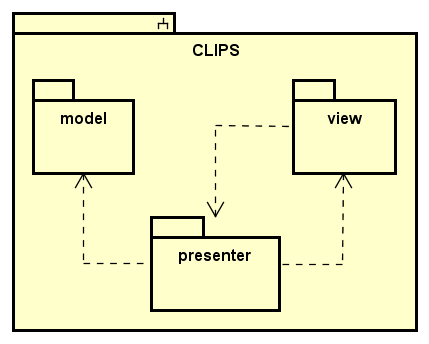
\includegraphics[scale=0.8]{img/package/CLIPS}
			\label{CLIPS}
			\caption{Diagramma dei package - sistema CLIPS}
		\end{figure}
		
	
	% componenti da esportare da Tracy
	
	
	
\end{document}